\documentclass[12pt,german]{article}

\usepackage[left=2cm, right=2cm, top=2cm, bottom=3.5cm, landscape=false]{geometry}

\usepackage{graphicx}
\usepackage{float}

\usepackage{tabularx}
\newcolumntype{R}{>{\raggedleft\arraybackslash}X}
\newcolumntype{L}{>{\raggedright\arraybackslash}X}
\newcolumntype{C}{>{\centering\arraybackslash}X}
\usepackage{booktabs}
\usepackage{dcolumn}

\usepackage[ngerman]{babel}

\usepackage{amsmath}

\title{\vspace{-1.5cm}Protokoll Gammaspektrometrie}
\author{Fuchs, Gutmann, Kosbab, Kowal, Steindorf, Fälker, Richter}

\begin{document}
    \maketitle
    \tableofcontents

    \section{Kurzbeschreibung des Versuches}
    \begin{itemize}
        \item Mithilfe von Cobalt-60 werden die Detektoren kalibriert, die Kalibrierung wird mit Cäsium-137 validiert.
        \item Auf Millimeterpapier wird die Linearität der Zuordnung von Kanallage zu Energie nachgewiesen.
        \item Es wird eine Kupfer-Probe für 10 Minuten aktiviert, anschließend mit dem Detektor ausgewertet und 10 Minuten später erneut ausgewertet.
        \item Im Reaktor wird die unbekannte Probe für 10 Minuten aktiviert.
        \item Die unbekannte Probe wird anhand der Fotopeaks ausgewertet, aufgrund verschobener Kalibrierung wird sie jedoch gegen eine neue unbekannte Probe ausgetauscht.
        \item Die neue Probe wird anhand der Fotopeaks identifiziert.
    \end{itemize}
    \newpage

    \section[Vergleich der Auflösung zwischen Halbleiter-Detektor und Szintillator]{Vergleich der Auflösung zwischen Halbleiter-Detektor und Szintillator am Beispiel von Cobalt-60}
    \begin{figure}[H]
        \begin{minipage}[t]{0.475\textwidth}
            \centering
            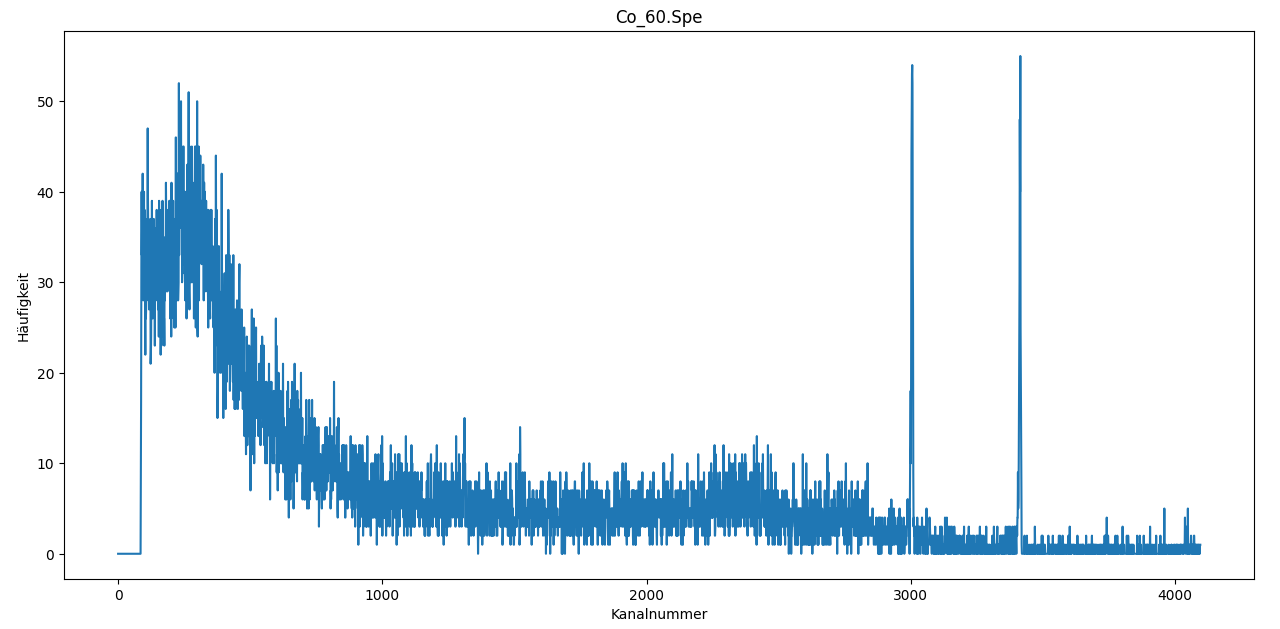
\includegraphics[width=1\textwidth]{pics/Co_60.png}
            \caption{Ge(Li) - Halbleiterdetektor}
        \end{minipage}
        \hfill
        \begin{minipage}[t]{0.475\textwidth}
            \centering
            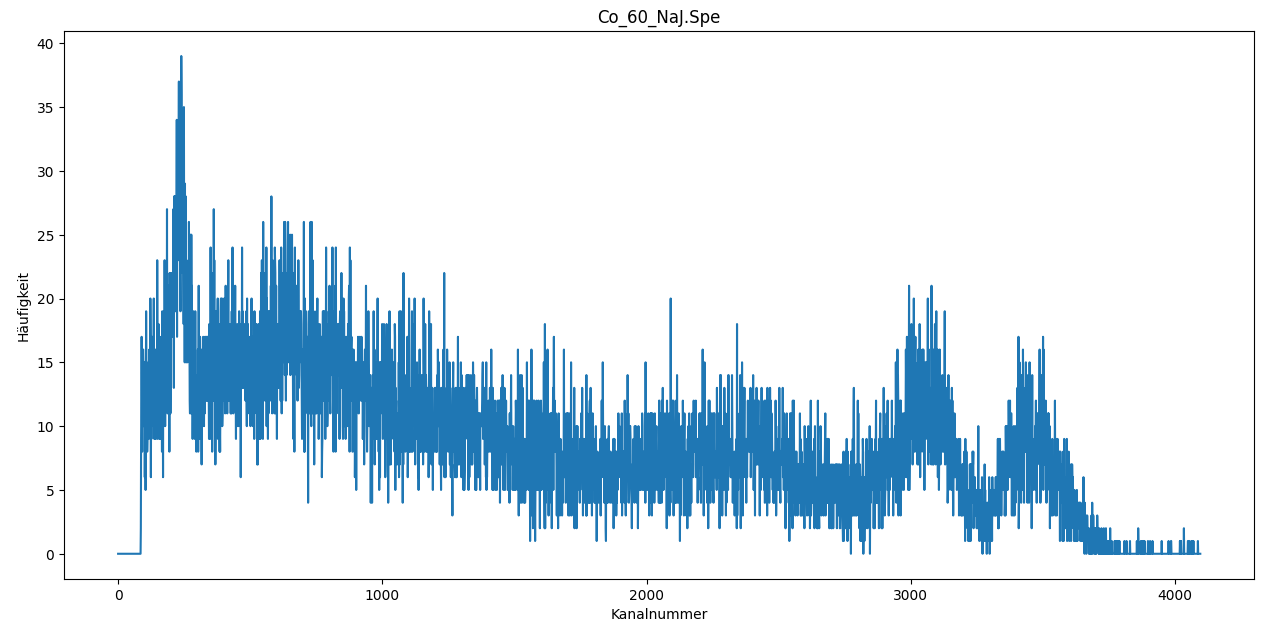
\includegraphics[width=1\textwidth]{pics/Co_60_NaJ.png}
            \caption{NaJ(TI) - Szintillator}
        \end{minipage}
    \end{figure}
    Es ist erkennbar, dass die Auflösung des Halbleiterdetektors höher ist als die des NaJ-Szintillators.
    Die Halbwertsbreite eines Peaks beträgt im NaJ-Szintillator ca. 200 Kanäle, im Halbleiterdetektor beträgt sie ca. 10 Kanäle.

    \section{Energiekalibrierung des Spektrometers mit Ge(Li)-Detektor}
    \begin{figure}[H]
        \centering
        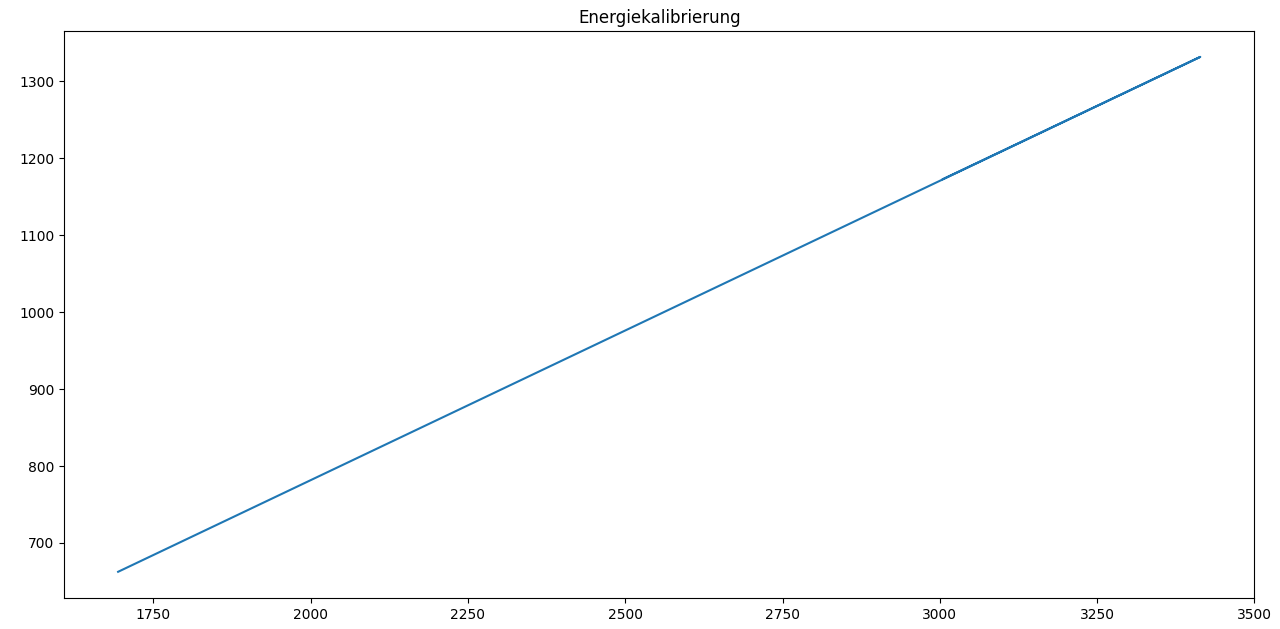
\includegraphics[width=0.7\textwidth]{pics/energiekalibrierung.png}
        \caption{Zusammenhang zwischen Kanallage und Energie}
        \label{fig:kanalenergie}
    \end{figure}
    Es werden die Kanallagen und Energien von Cobalt-60 und Cäsium-137 in einem Diagramm aufgetragen.
    Wie in Abbildung \ref{fig:kanalenergie} zu sehen ist besteht ein linearer Zusammenhang zwischen Kanal und Energie.

    \section{Auswertung von Kupfer}
    Artur ist ein Huso

    \section{Messung der ersten unbekannten Probe}
    
\end{document}